%%
%% The first command in your LaTeX source must be the \documentclass command.
%% nonacm option turns off ACM stuff like copyright notice and such
\documentclass[sigplan,screen,nonacm]{acmart}

%%
%% \BibTeX command to typeset BibTeX logo in the docs
\AtBeginDocument{%
  \providecommand\BibTeX{{%
    \normalfont B\kern-0.5em{\scshape i\kern-0.25em b}\kern-0.8em\TeX}}}

% painint TODOs red    
\newcommand\TODO[1]{\textcolor{red}{\emph{TODO #1}}}

%% end of the preamble, start of the body of the document source.
\begin{document}

%%
%% The "title" command has an optional parameter,
%% allowing the author to define a "short title" to be used in page headers.
\title[Hair Simulation]{Hair simulation using Position Based Dynamics}
\subtitle{5th semester Project Laboratory report}

%%
%% The "author" command and its associated commands are used to define
%% the authors and their affiliations.
%% Of note is the shared affiliation of the first two authors, and the
%% "authornote" and "authornotemark" commands
%% used to denote shared contribution to the research.
\author{Barnabás Börcsök}
% \authornote{BSc student}
\email{borcsok.barnabas@simonyi.bme.hu}
\affiliation{%
  \institution{Budapest University of Technology and Economics}
  \city{Budapest}
  \country{Hungary}
}


%%
%% By default, the full list of authors will be used in the page
%% headers. Often, this list is too long, and will overlap
%% other information printed in the page headers. This command allows
%% the author to define a more concise list
%% of authors' names for this purpose.
% \renewcommand{\shortauthors}{Trovato and Tobin, et al.}

%%
%% The abstract is a short summary of the work to be presented in the
%% article.
\begin{abstract}
    A self-assessment of the 5th semester Project Laboratory
    Project is presented in this article. My goal was to achieve hair simulation
    of acceptable quality both in terms of look and performance. Multiple
    approaches were considered before arriving at a Position Based Dynamics
    based solution. The simulation was implemented in C++ with the Open Graphics
    Library (OpenGL \footnote{\url{http://www.opengl.org}})
\end{abstract}

%%%
%%% The code below is generated by the tool at http://dl.acm.org/ccs.cfm.
%%% Please copy and paste the code instead of the example below.
%%%
\begin{CCSXML}
<ccs2012>
<concept>
<concept_id>10010147.10010371.10010352.10010379</concept_id>
<concept_desc>Computing methodologies~Physical simulation</concept_desc>
<concept_significance>300</concept_significance>
</concept>
</ccs2012>
\end{CCSXML}

\ccsdesc[300]{Computing methodologies~Physical simulation}
%%
%% Keywords. The author(s) should pick words that accurately describe
%% the work being presented. Separate the keywords with commas.
\keywords{hair simulation, position based dynamics, OpenGL}

%% A "teaser" image appears between the author and affiliation
%% information and the body of the document, and typically spans the
%% page.
\begin{teaserfigure}
  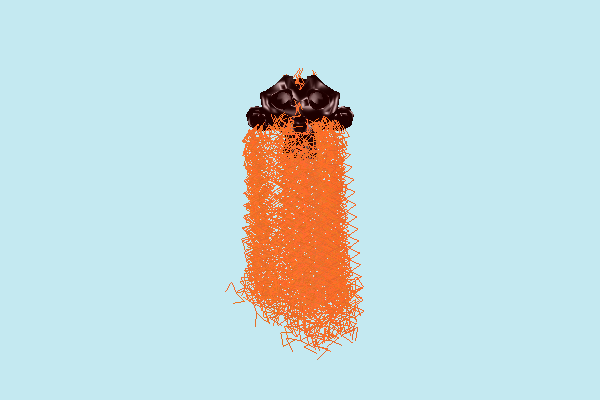
\includegraphics[width=\textwidth]{teaser.png}
  \caption{The achieved visual look}
  \Description{Using 400 hair pieces, with 25 particles on each piece of hair.}
  \label{fig:teaser}
\end{teaserfigure}

%%
%% This command processes the author and affiliation and title
%% information and builds the first part of the formatted document.
\maketitle

\section{Introduction}
In the 5th semester of their undergrad studies, BSc students from Budapest
University of Tehchnology and Economics embark on their first journey of
scientific research. I was always interested in and fascinated by computer 
graphics, it came naturally to choose a subject in this area. As I had little
 hands-on experience in this field, a long time had to be dedicated
to research and trying out different simulation methods.

The first of this paper reflects this, giving an overview of considered methods,
and other possible routes that could have been taken to implement hair
simulation.

\section{Overview of considered methods}

There were mainly three methods considered, two of them being substantially
different:


\subsection{Mass Spring System}
The whole idea of doing hair simulation as my project laboratory came from
\TODO{reference Pixar article and Khan Academy video} 

\begin{verbatim}
  \documentclass[STYLE]{acmart}
\end{verbatim}

\subsection{Position Based Dynamics}


\subsection{Follow the Leader}
The Dynamic Follow-The-Leader method outlined in \TODO{reference article}


%%
%% The acknowledgments section is defined using the "acks" environment
%% (and NOT an unnumbered section). This ensures the proper
%% identification of the section in the article metadata, and the
%% consistent spelling of the heading.
\begin{acks}
    To Dr. László Szécsi, associate professor at the Computer Graphics Group
    (Department of Control Engineering and Information Technology), whom I had
    the chance to consult with during the semester.
\end{acks}

%%
%% The next two lines define the bibliography style to be used, and
%% the bibliography file.
\bibliographystyle{ACM-Reference-Format}
\bibliography{references}

%%
%% If your work has an appendix, this is the place to put it.
\appendix

\section{Supplementary development}

\subsection{OBJ Reader}

Lorem ipsum dolor sit amet, consectetur adipiscing elit. Morbi
malesuada, quam in pulvinar varius, metus nunc fermentum urna, id
sollicitudin purus odio sit amet enim. Aliquam ullamcorper eu ipsum
vel mollis. Curabitur quis dictum nisl. Phasellus vel semper risus, et
lacinia dolor. Integer ultricies commodo sem nec semper.

\subsection{Recording the simulation on-the-fly}

Etiam commodo feugiat nisl pulvinar pellentesque. Etiam auctor sodales
ligula, non varius nibh pulvinar semper. Suspendisse nec lectus non
ipsum convallis congue hendrerit vitae sapien. Donec at laoreet
eros. Vivamus non purus placerat, scelerisque diam eu, cursus
ante. Etiam aliquam tortor auctor efficitur mattis.


\end{document}
\endinput
%%
%% End of file `documentation.tex'.
